\documentclass{article}

\usepackage{latexsym}
\usepackage{graphicx,caption}
\usepackage{mathptmx}
\usepackage{tikz}

\usepackage[margin=1in]{geometry}

%
%****************************************************************************
%  AUTHOR: You may want to use some of these packages. (Optional)
\usepackage{amsmath}
\usepackage{amsfonts}
\usepackage{amssymb}
\usepackage{amsbsy}
\usepackage{amsthm}
%****************************************************************************


% Custom commands
\newcommand{\mcomment}[2]{\textcolor{red}{#2}\marginpar[\color{red}\textbf{\hskip 60pt {#1}} $\Leftarrow$]{{\color{red}\textbf{#1 Note}}}}
\newcommand{\annotate}[1]{{\color{blue}#1}}
\newcommand{\annotatenew}[1]{{\color{red}#1}}

% Added packages
\usepackage[linesnumbered,lined,noline,ruled,noend]{algorithm2e}
\usepackage{textcomp}
\usepackage{multirow}
\usepackage{epsfig,graphicx}
\usepackage{amsmath,amsfonts,amssymb,amsthm}
\usepackage{booktabs}
\usepackage{paralist}
\usepackage[pdftex,colorlinks=true,urlcolor=blue,citecolor=black,anchorcolor=black,linkcolor=black]{hyperref}
\usepackage[capitalize]{cleveref}
\usepackage{fancyhdr}
\usepackage{subcaption}

%%% Math environments
\newtheorem{theorem}{Theorem}
\theoremstyle{definition}
\newtheorem{definition}{Definition}

\theoremstyle{example}
\newtheorem{example}{Example}

\theoremstyle{example}
\newtheorem{remark}{Remark}

\theoremstyle{example}
\newtheorem{assumption}{Assumption}

% Neat trick for (scaled) ceiling and floor functions
\usepackage{mathtools}
\DeclarePairedDelimiter\ceil{\lceil}{\rceil}
\DeclarePairedDelimiter\floor{\lfloor}{\rfloor}


\title{Dynamic Non-Uniform Randomization in Asynchronous Linear Solvers}
\author{Evan Coleman \and Masha Sosonkina}
\date{}



%#########################################################
%*
%*  The Document.
%*
\begin{document}
	
\maketitle

\begin{abstract}
	Asynchronous iterative methods present a mechanism to improve the performance of algorithms for highly parallel computational platforms by removing the overhead associated with synchronization among computing elements. This paper considers a class of asynchronous iterative linear system solvers that employ randomization to determine the component update orders; specifically focusing on the effects of both using non-uniform distributions in the selection of which block to work on, and on dynamically changing the ranking throughout the iteration. Results show that using distributions favoring the selection of components with a larger contribution to the residual can lead to a faster convergence compared to selecting components uniformly. 
\end{abstract}
% Keywords
\noindent
{\em {\bf Keywords:} asynchronous iteration, linear solver, randomized linear algebra}


%------------------------------------------------------------------------------
% Introduction
%
\section{Introduction}
\label{sec:intro}

Asynchronous iterative methods describe a class of parallel iterative algorithms where each computing element is allowed to perform its task without waiting for updates from any of the other processes. Asynchronous iteration is often applied to the parallel solution of fixed point problems, whereby a fixed point iteration, $x^{(k+1)} = G(x^{(k)})$, is updated in an asynchronous manner. This class of problems has been used in a wide variety of applications including: the solution of linear systems \cite{recht2011hogwild}, the preconditioning of linear solvers \cite{chow2015fine}, optimization \cite{srivastava2011distributed}, and techniques for solving partial differential equations \cite{magoules2015asynchronous}, among many others. 

Asynchronous linear solvers tend not to converge to high precision as quickly as their Krylov subspace counterparts, however they can converge very quickly to a low level of accuracy \cite{avron2015revisiting}. This loss of accuracy may cause the use of asynchronous linear solvers to be suboptimal for some applications, but the fact that they are able to reach an approximate solution quickly opens up several other application areas. For example, possible use cases include using the asynchronous linear solver as a preconditioner to a traditional Krylov subspace solver, to solve systems that only require lower accuracy solutions (e.g. big data, machine learning, etc), or else as a smoother to multigrid methods. In any of these use cases, the acceleration of this class of algorithms has an impact across a wide variety of domain areas in science and engineering.

One approach to potentially improving the performance of asynchronous linear solvers is to have each processor select randomly the (block of) components it updates next, as opposed fixing an update order before the iteration commences. This approach has been studied previously for the case where the random selection is done uniformly \cite{strikwerda2002probabilistic,avron2015revisiting}. A non-uniform random selection is considered in both \cite{leventhal2010randomized} and \cite{griebel2012greedy} for the case of synchronous algorithms, however, in both of those studies the update order remains fixed throughout the algorithm and does not dynamically change over the course of algorithm. The main contribution of this work is to analyze the potential performance benefit for asynchronous linear solvers of randomly selecting the next component to update using a non-uniform distribution, and to evaluate the viability of changing the update order throughout the iteration. This dynamic updating procedure is motivated in part by weighted stationary solvers, such as the Southwell iteration, that select the component with the largest contribution to the residual at each iteration and which are typically able to converge in fewer iterations than traditional Jacobi or Gauss-Seidel relaxation schemes. Both the situation in the traditional Southwell algorithm as well as the situation generated by the algorithm studied here have to establish that the extra computational time required to dynamically select components that contribute more to the residual is overcome by the savings in total iterations in order to establish the algorithm as viable.

Note that as shown by \cite{griebel2012greedy}, all of the results presented here extend naturally to Hilbert spaces, however, the analysis is limited to real matrices in finite dimensional Euclidean space. The structure of the rest of this paper is as follows: first, \cref{sect:related-work} provides information on related studies, and next \cref{sect:asynchronous-iterative-methods} overviews asynchronous iterative methods, including the specific assumptions that are made here. \Cref{sect:randomized-linear-solvers} discusses the use of asynchronous, randomized linear solvers and proposes and analyzes variations of the randomization procedure, and \cref{sect:summary-future-work} concludes.


%------------------------------------------------------------------------------
% Related Work
%
\section{Related Work}
\label{sect:related-work}

The Department of Energy has commissioned two very detailed reports about the progression towards exascale level computing; one from a general computing standpoint conducted by \cite{ashby2010ascac}, and a report aimed specifically at applied mathematics for exascale computing by \cite{dongarra2014applied}; both of which emphasize the importance of developing scalable algorithms moving forward towards exascale platforms. Development of scalable applications on a large scale starts with modifying algorithms that form the basis for those application, and the stationary iterative methods examined here (e.g., Jacobi, Gauss-Seidel, block variants) form an important aspect of many preconditioning techniques for Krylov subspace methods, as well as commonly acting as smoother in multigrid methods.

Several recent studies focus on improving scalability by attempting to remove the synchronization delay: a fine-grained algorithm for computing incomplete LU factors for the purposes of preconditioning of linear solvers was created by \cite{chow2015fine}, an optimization technique based upon an asynchronous approach to stochastic gradient descent was created by \cite{recht2011hogwild}, and the efficacy of  asynchronous multigrid smoothers was explored for CFD applications in \cite{kashi2018asynchronous}. The use of randomization in linear algebra has found use in a variety of areas including transforming linear systems using Random Butterfly Transformations to eliminate (with probability 1) the need for pivoting. This has been used to aid in the performance of direct solvers for dense matrices by \cite{parker1995random}, and later adopted for sparse matrices by \cite{baboulin2014using}. Other examples include the random component selection in stochastic gradient descent methods, including an early study \cite{srivastava2011distributed} that incorporates asynchronous computation. More pertinent to the topic studied here, randomized linear relaxation based solvers have been studied in the past by \cite{strikwerda2002probabilistic} who extend the original asynchronous model presented by \cite{chazan1969chaotic} to allow component choice and (theoretical) delay to be based upon probability distributions.

The thrust of this paper is to incorporate asynchronous computation with randomization in such a way that accelerates convergence relative to uniformly selecting the next component to update. To this end, a greedy approach, similar in spirit to the Southwell iteration, is used. A Southwell oriented approach has been extended to the case of parallel asynchronous solvers previously by \cite{wolfson2017distributed}, whereby an equation is relaxed if it has the largest residual among all coupled equations. 




%------------------------------------------------------------------------------
% Stationary/Relaxation Methods
%
\section{Asynchronous Iterative Methods}
\label{sect:asynchronous-iterative-methods}

In asynchronous computation, each part of the problem is updated such that no information from other parts is needed while each individual computation is performed. This allows each processor to act independently. The model that is shown here to provide a basis for asynchronous computation comes mainly from \cite{frommer2000asynchronous}. To start, consider a fixed point iteration with the function, $G: D \rightarrow D$. Given a finite number of processors ${P_1, P_2, \ldots, P_p}$  each assigned to a block {\cal B} of components ${B_1, B_2, \ldots, B_m}$, the computational model can be stated in \cref{algo:computational-model-1}.

%The algorithm2e code for the Asynchronous Iterative Computational Model (Frommer & Szyld 2000)
\begin{algorithm}
	\DontPrintSemicolon
	\For {each processing element $P_{l}$} {
		\For {$i = 1, 2, \ldots$ until convergence} {
			Read $x$ from common memory \;
			Compute $x_j^{i+1} = G_j(x)$ for all  $j \in {\cal B}_{l}$ \;
			Update $x_j$ in common memory with $x_j^{i+1}$ for all
			$j \in {\cal B}_{l}$ \;
		}
	}
	\caption{General Computational Model}
	\label{algo:computational-model-1}
\end{algorithm}

If each processors ($P_l$) waits for the other processors to finish each update, then the model describes a parallel synchronous form of computation. If no order is established for the processors, then the computation is asynchronous. At the end of an update by processor $p$, the components associated with the block $B_p$ will be updated. This results in a vector, $x = (x_1^{s_1(k)}, x_2^{s_2(k)}, \ldots, x_m^{s_m(k)})$ where $s_l(k)$ indicates how many times component $l$ has been updated, and $k$ is a global iteration counter. A set of indices $I^k$ contains the components that were updated on the $k^{th}$ iteration. Given these definitions, the three following conditions provide a framework for asynchronous computation:

\begin{definition}
	\label{def:asynchronous-model}
	If the following three conditions hold:
	\begin{enumerate}
		\item	$s_i(k) \leq k - 1$, {\em i.e., only components that have finished computing are used in the current approximation.}
		\item	$\lim_{k\rightarrow \infty} s_i(k) = \infty$, {\em i.e., the newest updates for each component are used.}
		\item	$|{k \in \mathbb{N}: i \in I^k}| = \infty$, {\em i.e., all components will continue to be updated.}
	\end{enumerate}
	Then given an initial $x^0 \in D$, the iterative update process defined by,
	\[ x_i^{(k)} =
	\begin{cases}
	x_i^{(k-1)} 		& 	i \notin I^k \\
	G_i(x^{(k)}) 		&	i \in    I^k
	\end{cases}
	\]
	where the individual functions $G_i(\vec{x})$ use the latest updates available, is called an asynchronous iteration.
\end{definition}

This basic computational model (i.e. the combination of \cref{algo:computational-model-1} and \cref{def:asynchronous-model} together) allows for many different results on fine-grained iterative methods.


%------------------------------------------------------------------------------
% Randomized Parallel Southwell Algorithm
%
\section{Randomized Linear Solvers}
\label{sect:randomized-linear-solvers}

Relaxation methods have been the focus of many studies related to asynchronous iterations starting with \cite{chazan1969chaotic} and \cite{baudet1978asynchronous}. They are typically used to solve linear systems of the form $Ax = b$ and can be written as fixed point iterations that can be expressed as
\begin{equation}
\label{eq:fixed-point-iteration-matrix}
x^{k+1} = C x^k + d\; ,
\end{equation}
\noindent
where $C$ is the $n\times n$ iteration matrix, $x$ is an $n$-dimensional vector that represents the solution, and $d$ is another $n$-dimensional vector that can be used to help define the particular problem at hand. The Jacobi method is a relaxation method that can be used in an asynchronous manner and the update for a given component $x_i$ can be expressed as
\begin{equation}
\label{eq:element-wise-jacobi}
x_i = \frac{-1}{a_{ii}}\left[\sum_{j\neq i} a_{ij}x_j - b_i \right].
\end{equation}
\noindent
This iteration can give successive updates to the $x_i$ component in the solution vector. In synchronous computing environments, each update to an element of the solution vector, $x_i$, is computed sequentially using the same data for the other components of the solution vector (i.e., the values for $x_j$ in \cref{eq:element-wise-jacobi}). Conversely, in an asynchronous computing environment, each update to an element of the solution vector occurs when the computing element responsible for updating that component is ready to write the update to memory and the other components used are simply the latest ones available to the computing element. Expressing \cref{eq:element-wise-jacobi} in a block form similar to \cref{eq:fixed-point-iteration-matrix} gives an iteration matrix of $C = -D^{-1}(L+U)$ where $D$ is the diagonal portion of $A$, and $L$ and $U$ are the strictly lower and upper triangular portions of $A$ respectively. Convergence of asynchronous fixed point methods of the form presented in \cref{eq:fixed-point-iteration-matrix} is determined by the spectral radius of the iteration matrix, $C$. 

\begin{theorem}
	\label{th:fixed-point-convergence}
	For a fixed point iteration of the form given in \cref{eq:fixed-point-iteration-matrix} that adheres to the	asynchronous computational model provided by \cref{algo:computational-model-1} and \cref{def:asynchronous-model}, if the spectral radius of $C$, $\rho(|C|)$, ls less than one, then the iterative method will converge to the fixed point solution.
\end{theorem}

Asymptotic results such as this, i.e. that guarantee eventual convergence but offer no guarantee as to the rate of that convergence, exist for many variants of the iteration described above (see \cite{frommer2000asynchronous} for a summary). The use of randomization in asynchronous linear solvers allows for the possibility of statements concerning the rate of convergence to be made. Leventhal and Lewis introduced a randomized Gauss-Seidel method \cite{leventhal2010randomized} building off of the randomized Kaczmarz algorithm proposed by Strohmer and Vershynin \cite{strohmer2009randomized}. The analysis was generalized by Griebel and Oswald who also added a new parameter that allows for both over and under relaxation \cite{griebel2012greedy}. The work that much of the analysis in the paper is based off of is due Avron, Druinsky, and Gupta who build upon the analysis and explicitly analyze the case of asynchronous computation \cite{avron2015revisiting}.  

Each of the methods select the vector component to update (see \cref{eq:element-wise-jacobi}) from a random distribution instead of either sequentially looping through the available components or by tying the updates for a single component to a particular processor. In a traditional parallelization of either a synchronous or asynchronous linear solver, processor $j$ is responsible for updating component $j$; the asynchronous variant allows processor $j$ to continue to compute relaxations for the component assigned to it regardless of the state of the other processors. The use of randomization in the selection of which component to update allows for the possibility of any processor updating any component.

In a randomized asynchronous linear solver, when a processor finishes computing an update to a component, it writes the update to shared memory and then randomly draws the next component to update from the list of all available components. In practice, a processor will often select a contiguous block of components to update as opposed to an individual row. The updating of components inside of the block can be done in a variety of different ways, but will often be done sequentially using a traditional Gauss-Seidel algorithm. Throughout this analysis, a {\em consistent read} (using the terminology from \cite{avron2015revisiting}) is assumed; whereby no processor is partway through writing a block to memory while another processor is reading it. This could cause an update to be performed using a vector, $x$, that never existed. Though the asynchronous nature of the computation allows the possibility of an inconsistent read from memory without using atomic operations to enforce safety, Avron et al point out that such a read is very uncommon in practice \cite{avron2015revisiting}.

In the randomized asynchronous linear solvers proposed to date, this random selection is always done using either uniform random number generation, or with a probability proportional to a row norm of the matrix $A$. Leventhal and Lewis cite Fourier analysis \cite{leventhal2010randomized} as an application area that can benefit from this type of weighting; however, there is no reason to expect improved behavior for an arbitrary problem. A major point of exploration here is to investigate the feasibility of using non-uniform distributions in the selection of which component to update.

\subsection{Improved Randomized Linear Solvers}
\label{sect:improved-randomized-linear-solvers}

The Southwell algorithm \cite{southwell1946relaxation} works similar to Jacobi by relaxing a single equation at a time, but chooses the equation with the largest local residual. This difference allows the Southwell algorithm to often converge in fewer iterations than Jacobi, but raises the expense of computing an update since the local residuals need to be stored and ranked at each iteration. For example, after a given iteration, the Southwell algorithm will choose the component that contributes the most to the global residual to update; in order to do this, the algorithm must rank the residuals from largest to smallest.

\begin{enumerate}
	\item pick a random $j \in \{1, 2, \ldots, n\}$ under the assumption there are $n$ equations in the matrix
	\item read the corresponding entries of $A, x, b$
	\item perform the relaxation for equation $x_j$
	\item update the data for $x_j$
\end{enumerate}

Using the insight from the Southwell algorithm and the success found in the parallel Southwell implementations~\cite{wolfson2016reducing,wolfson2017distributed}, the idea behind the randomized linear solvers considered here is for each processor to select the next component it is responsible for updating randomly, using a distribution that more heavily weights selection of components that contribute more to the global residual.  Pseudo-code for a randomized variant is provided by \cref{algo:randomized-computational-model}, which is the same as the one for the randomized asynchronous Jacobi presented in \cite{avron2015revisiting}, where a  uniform distribution over $\{1, 2, \ldots, n\}$ is studied. The key difference of the present work is that here non-uniform distributions  in~\cref{alg:pickrandom} of~\cref{algo:randomized-computational-model} are investigated. 

\begin{algorithm}[ht!]
	\DontPrintSemicolon
	\For {each processing element $P_{l}$} {
		\For {$i = 1, 2, \ldots$ until convergence} {
			Pick $j \in \{1, 2, \ldots, n\}$ using a given probability distribution \; \label{alg:pickrandom}
			Read the corresponding entries of $A, x, b$ \label{step:read}\;
			Perform the relaxation for equation $x_j$ \label{step:relax}\;
			Update the data for $x_j$ \;
		}
	}
	\caption{Generic Randomized Linear Solver}
	\label{algo:randomized-computational-model}
\end{algorithm}

The goal behind many of the proposed modifications to the Generic Randomized Linear Solver presented in \cref{algo:randomized-computational-model} is that relaxing the components with a more significant contribution to the global residual may reduce the total number of iterations required. Motivation for this comes from a myriad of different studies, see for instance the paper by Nutini et al that shows that for some cases (Gauss-)Southwell selection can converge faster than uniform random selection for coordinate descent \cite{nutini2015coordinate}. In general, the improvement in convergence will have to be shown to be significant enough to offset the extra computational and communication cost associated with storing and ranking all of the local residuals. 

In an effort to simulate the effect of the Southwell algorithm using randomized asynchronous solvers,  the {\em local residuals} associated with each equation (or block of equations) are ranked and sorted, and the selection of the next equation (i.e., component) to update is performed using a non-uniform distribution that forces the random selection to pick components with larger local residuals more frequently. The Southwell algorithm \cite{southwell1946relaxation} works similar to Jacobi by relaxing a single equation at a time, but chooses the equation with the largest local contribution to the residual. For a given row (or block of rows) $i$, this local contribution is defined to be

\begin{equation}
r_i^{(k)} = b_i - Ax_i^{(k)}
\end{equation}

\noindent
at iteration $k$. This difference allows the Southwell algorithm to often converge in fewer iterations than Jacobi, but raises the expense of computing an update since the local residuals need to be stored and ranked at each iteration. For example, after a given iteration, the Southwell algorithm will choose the component that contributes the most to the global residual to update; in order to do this, the algorithm must rank the residuals from largest to smallest. Since ranking and sorting local residuals can be expensive, the periodicity with which this is done contributes to the overall efficiency of the algorithm. Previously in \cite{jensen2018using}, the authors have studied a balance between computational effort spent performing relaxations compared with other algorithmic operations and communications in asynchronous methods.

Before commencing analysis of the new variants, a brief review of existing results for similar algorithms is provided. The main goal of this type of analysis is first to verify convergence of the algorithm, and then provide convergence rate analysis when possible. The first result is due to Leventhal and Lewis \cite{leventhal2010randomized}. In this variant of the algorithm, the component $j$ is chosen with probability,
	\begin{equation}
		\mathbb{P}\{j = k\} = \frac{a_{kk}}{tr(A)}.
	\end{equation}
\noindent
Given this, the following result from \cite{leventhal2010randomized} establishes a bound on convergence rate. Note that this algorithm is analyzed from a deterministic point of view in \cite{leventhal2010randomized} that neglects the effects of asynchronous parallelism.

\begin{theorem}[Leventhal, Lewis]
	If $A$ is symmetric and positive-definite, then the variant of \cref{algo:randomized-computational-model} due to Leventhal and Lewis described above satisfies the property,
		\begin{equation}
			\mathbb{E}[\Vert x^{(j)} - x^* \Vert_A^2] \leq \left(1 - \frac{1}{\Vert A^{-1} \Vert_2 tr(A)}\right) \Vert x^{(j-1)} - x^* \Vert_A^2
		\end{equation}
	which shows that the iteration converges linearly in the $A$-norm.
\end{theorem}

The next result, due to Griebel and Oswald \cite{griebel2012greedy}, adds an over/under relaxation parameter, $\beta$, to the algorithm. Note that \cref{step:relax} of \cref{algo:randomized-computational-model} can be written,

\begin{equation}
	x_j^{(i+1)} = x_j^{(i)} + \frac{\beta}{a_{ii}} r_j^{(i)}
\end{equation}
\noindent
That is, the relaxations performed in \cref{step:relax} of \cref{algo:randomized-computational-model} are weighted by a step size parameter before they are applied. This new algorithm serves as a starting point for the analysis continued below and is expressed explicitly in \cref{algo:randomized-computational-model2}.

\begin{algorithm}[ht!]
	\DontPrintSemicolon
	\For {each processing element $P_{l}$} {
		\For {$i = 1, 2, \ldots$ until convergence} {
			Pick $j \in \{1, 2, \ldots, n\}$ using a given probability distribution \; \label{alg:pickrandom2}
			Read the corresponding entries of $A, x, b$ \label{step:read2}\;
			Compute $x^{(i)}_j = x^{(i-1)}_j + \frac{\beta}{a_{ii}} r^{(i)}_j$ \;
			Update the data for $x^{(i)}_j$ \;
		}
	}
	\caption{Updated Randomized Linear Solver}
	\label{algo:randomized-computational-model2}
\end{algorithm}

In this case, linear convergence is maintained, but the bound changes slightly. The corresponding result is due to Griebel and Oswald \cite{griebel2012greedy} and is provided below.

\begin{theorem}[Griebel, Oswald]
	If $A$ is symmetric and positive-definite, then the variant of \cref{algo:randomized-computational-model} due to Griebel and Oswald described above satisfies the property,
		\begin{equation}
			\mathbb{E}[\Vert x^{(j)} - x^* \Vert_A^2] \leq \left(1 - \frac{\beta (2 - \beta)\lambda_{min}}{tr(A)}\right)^m \Vert x^{(0)} - x^* \Vert_A^2
		\end{equation}
	which shows that the iteration converges linearly in the $A$-norm.
\end{theorem}
	

When the selection in \cref{alg:pickrandom} of \cref{algo:randomized-computational-model2} is done using a combination of: a uniform distribution, an asynchronous mode of computation (with a consistent read model), $A$ taken to be symmetric and positive-definite, and there is a bound, denoted $\tau$, on how out-of-date information for any component can be, then the following result gives a bound on convergence rate.

\begin{theorem}[Avron, Druinsky, Gupta]
	For an arbitrary starting vector, $x^{(0)}$, if $\rho = \frac{1}{n} \Vert A \Vert_\infty$, then if $2\rho \tau < 1$ the following hold:
		\begin{enumerate}
			\item For every $m \geq \frac{log(1/2)}{log(1-\lambda_{max}/n)} \approx \frac{0.693n}{\lambda_{max}}$,
					\begin{equation}
						\mathbb{E}[\Vert x^{(m)} - x^* \Vert_A^2] \leq \left( 1 - \frac{\nu_\tau}{2\kappa(A)}\right) \cdot \mathbb{E}[\Vert x^{(0)} - x^* \Vert_A^2]
					\end{equation}
				where
					\begin{equation}
						\nu_\tau = 1 - 2 \rho \tau
					\end{equation}
			\item Let $T_0 = \ceil*{\frac{log(1/2)}{log(1 - \lambda_{max}/n)}}$ and $T = T_0 + \tau$. For every $m \geq rT (r = 1, 2, \ldots)$,
					\begin{equation}
						\mathbb{E}[\Vert x^{(m)} - x^* \Vert_A^2] \leq \left( 1 - \frac{\nu_\tau}{2\kappa(A)}\right) \left( 1 - \frac{\nu_\tau(1 - \lambda_{max}/n)^\tau}{2\kappa(A)} + \chi \right) \mathbb{E}[\Vert x^{(0)} - x^* \Vert_A^2]
					\end{equation}
				where 
					\begin{equation}
						\chi = \frac{\rho \tau^2 \lambda_{max}(1 - \lambda_{max}/n)^{-2\tau}}{n}
					\end{equation}			
			\end{enumerate}
\end{theorem}

\subsection{New Variants of Randomized Linear Solvers}
\label{sect:new-variants-of-randomized-linear-solvers}

The analysis for the new variants of the algorithm picks up from this point. For the following discussion, assume that $A$ is symmetric and positive-definite. All of these variants are built around exploiting a Southwell like selection of the next component $j$. As a foundation for the randomized variants, a Southwell-Schwarz method due to Griebel and Oswald is presented first in \cref{algo:southwell-schwarz-linear-solver}.

\begin{algorithm}[ht!]
	\DontPrintSemicolon
	\For {each processing element $P_{l}$} {
		\For {$i = 1, 2, \ldots$ until convergence} {
			Pick an index, $j \in \{1, 2, \ldots, n\}$ such that $r_j^{(i)} \geq \alpha \max_k r_k^{(i)}$ \; \label{alg:picksouthwell}
			Read the corresponding entries of $A, x, b$ \label{step:read25}\;
			Compute $x^{(i)}_j = x^{(i-1)}_j + \frac{\beta}{a_{ii}} r^{(i)}_j$ \;
			Update the data for $x^{(i)}_j$ \;
		}
	}
	\caption{Southwell-Schwarz Linear Solver}
	\label{algo:southwell-schwarz-linear-solver}
\end{algorithm}

The procedure detailed in \cref{algo:southwell-schwarz-linear-solver} selects (non-randomly) an index that is close to being the largest contributor to the residual. This algorithm makes use of a weakness parameter, $\alpha$ with $0 \leq \alpha \leq 1$, whereby if $\alpha = 0$ any component $j$ can be selected, and if $\alpha = 1$ the original Southwell method (where only the single component with the largest contribution to the residual is eligible to be selected) is obtained. The method for choosing the index from among the allowed indices defined by the weakness parameter $\alpha$ is not specified explicitly in the original paper \cite{griebel2012greedy}. Corresponding to this algorithm is another result detailing linear convergence with no reliance on the expected outcome since the algorithm no longer relies upon random processes.

\begin{theorem}[Griebel, Oswald]
\label{th:southwell-schwarz}
	If $A$ is symmetric and positive-definite, then the variant of \cref{algo:randomized-computational-model} due to Griebel and Oswald described above satisfies the property,
	\begin{equation}
	\Vert x^{(j)} - x^* \Vert_A^2 \leq \left(1 - \frac{\alpha^2 \beta (2 - \beta)\lambda_{min}}{tr(A)}\right)^m \Vert x^{(0)} - x^* \Vert_A^2
	\end{equation}
	which shows that the iteration converges linearly in the $A$-norm.
\end{theorem}

Updating all the residuals every iteration in order to make this selection as defined likely introduces too much computational overhead to be of practical use. Periodically ranking the residuals and setting $\alpha$ in a problem specific manner creates a dynamically changing list of indices eligible for selection. All of these eligible indices correspond to components with larger local contribution to the global residual. The thrust of the new algorithms is to focus on techniques that achieve this dynamic focus on components that contribute more to the residual, but to do it in a different manner that no longer excludes a large set of indices and that more explicitly defines the method for selecting the next index to use from the prescribed list. To to do this, the randomized variants will be modified to use distributions that are weighted to more often select components with larger contribution to the residual. This is motivated by the case presented in \cref{example:sorted-residuals}.

\begin{example}
\label{example:sorted-residuals}
	Consider the two dimensional finite-difference discretization of the Laplacian, $-\Delta u = f$, with Dirichlet boundary conditions taken over a $10 \times 10$ grid. This results in 100 different components to update. The initial residuals for each component are shown in \cref{fig:initial-residuals-laplacian} both unsorted (left) and sorted from largest to smallest (right). From \cref{sfig:sorted-residuals}, it may be clearly seen that using a non-uniform distribution that favors specific parts of the ``slope'' is effectively possible, and prioritizing the updates of the components contributing the most to the global residual may be beneficial to convergence similar to the Southwell method.
	
	\begin{figure}[ht!]
		\centering
		\begin{subfigure}{0.45\textwidth}
			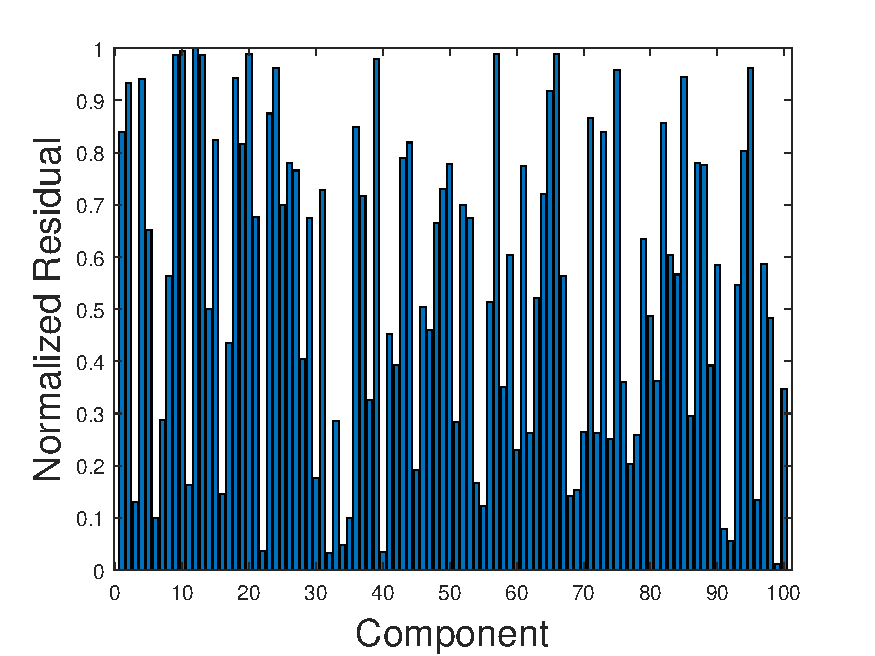
\includegraphics[width=\textwidth]{images/init_resids_10x10.pdf}
			\caption{Unsorted Residuals}
			\label{sfig:unsorted-residuals}
		\end{subfigure}
		\begin{subfigure}{0.45\textwidth}
			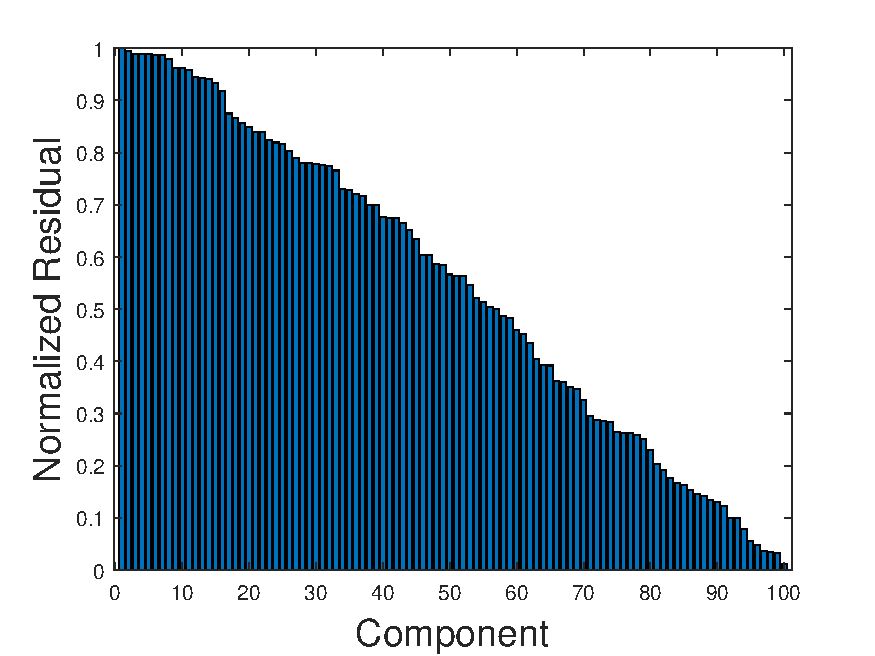
\includegraphics[width=\textwidth]{images/init_resids_10x10_sorted.pdf}
			\caption{Sorted Residuals}
			\label{sfig:sorted-residuals}
		\end{subfigure}
		\caption{Initial component residuals ($r_i / \max (r_i)$).}
		\label{fig:initial-residuals-laplacian}
	\end{figure}
\end{example}

The sorted residuals in \cref{sfig:sorted-residuals} indicate that a non-uniform distribution that targets components with larger contribution to the residual, but not necessarily restricted to the component with the single largest contribution, could be beneficial. For example, \cref{fig:distribution-residuals} shows an overlay of exponential distributions on the sorted, normalized component residuals at initialization, after each component has been relaxed 10 times, and after convergence has been achieved.

\begin{figure}[ht!]	
	\begin{subfigure}{0.33\linewidth}
		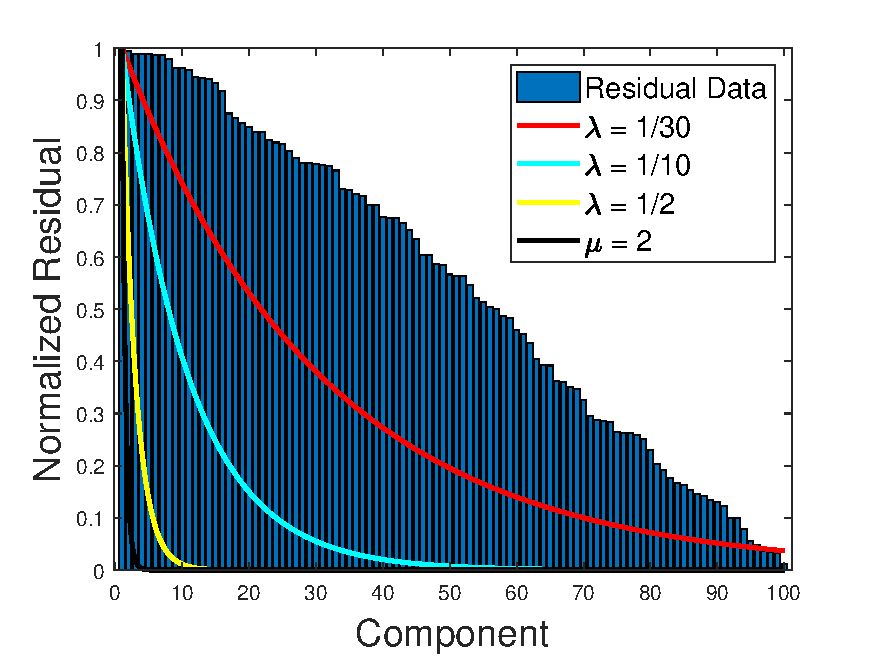
\includegraphics[width=\textwidth]{images/exp_dist_overlay_init.pdf}
		\caption{Initial residuals}
		\label{exp_dist_init}
	\end{subfigure}		
	\begin{subfigure}{0.33\linewidth}
		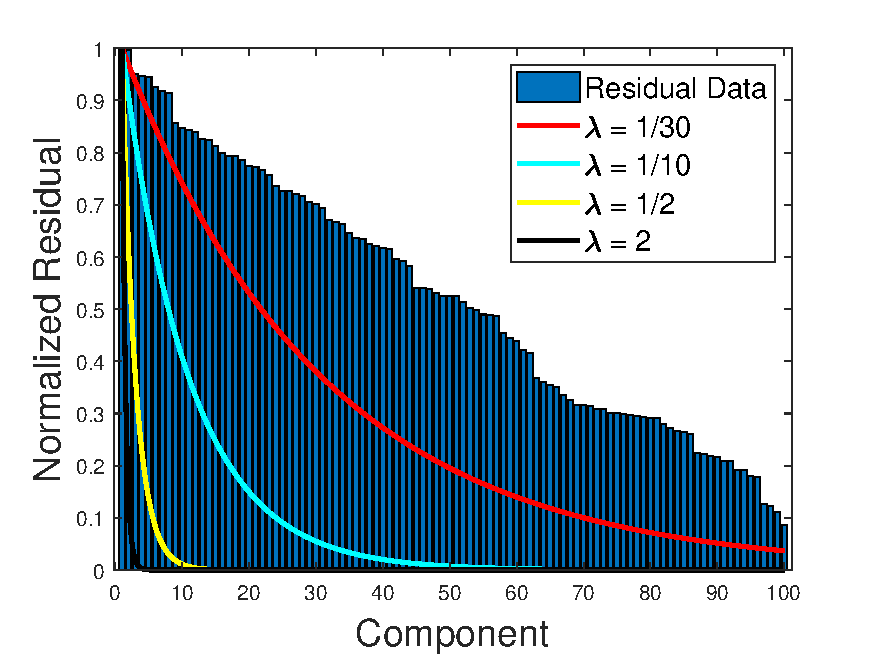
\includegraphics[width=\textwidth]{images/exp_dist_overlay_10iter.pdf}
		\caption{Residuals at 10 iterations}
		\label{exp_dist_10iter}
	\end{subfigure}		
	\begin{subfigure}{0.33\linewidth}
		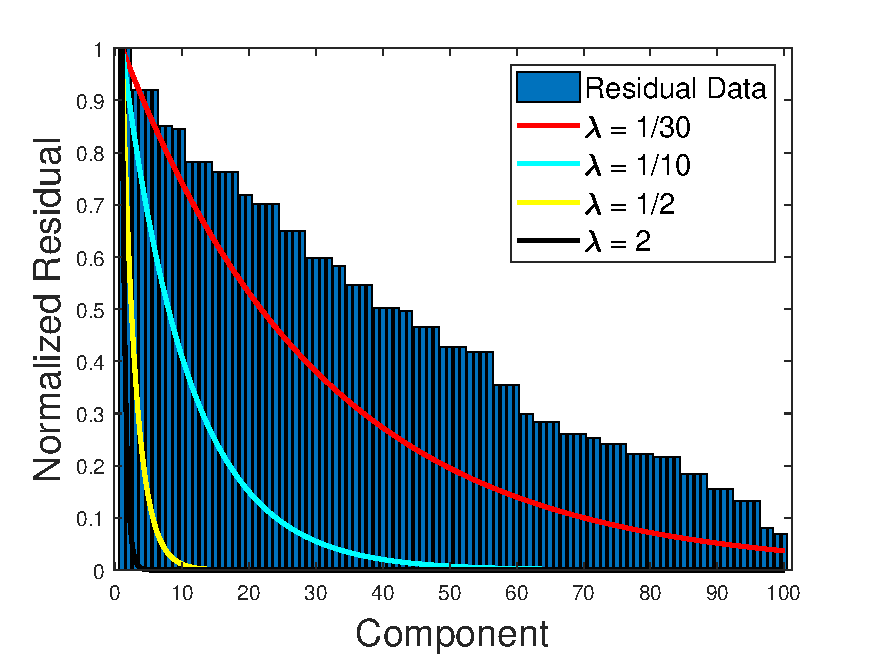
\includegraphics[width=\textwidth]{images/exp_dist_overlay_final.pdf}
		\caption{Final residuals}
		\label{exp_dist_final}
	\end{subfigure}
	
	\caption{Sorted residuals ($r_i / \max (r_i)$) with exponential distributions for reference.}
	\label{fig:distribution-residuals}
\end{figure}

The a non-dynamic variant of the algorithm corresponding to using a weighted probability distribution (such as an exponential distribution) is given in \cref{algo:randomized-computational-model3}.

\begin{algorithm}[ht!]
	\DontPrintSemicolon
	Compute component residuals \;
	Rank and sort the component residuals \;
	\For {each processing element $P_{l}$} {
		\For {$i = 1, 2, \ldots$ until convergence} {
			Pick $j \in \{1, 2, \ldots, n\}$ using a weighted probability distribution \; \label{alg:pickrandom3}
			Read the corresponding entries of $A, x, b$ \label{step:read3}\;
			Compute $x^{(i)}_j = x^{(i-1)}_j + \frac{\beta}{a_{ii}} r^{(i)}_j$ \label{step:update} \;
			Update the data for $x^{(i)}_j$ \;
		}
	}
	\caption{Weighted Randomized Linear Solver}
	\label{algo:randomized-computational-model3}
\end{algorithm}

However, one of the points of emphasis for the algorithms developed in this paper was the focus on dynamically changing the component selection process as the iteration progresses. To this end, each time a component residual is calculated (c.f. \cref{step:update} of \cref{algo:randomized-computational-model3}) the ranked and sorted list of component residuals can be updated. This variation is shown in \cref{step:dynamic-update} of \cref{algo:randomized-computational-model4}.

\begin{algorithm}[ht!]
	\DontPrintSemicolon
	Compute component residuals \;
	Rank and sort the component residuals \;
	\For {each processing element $P_{l}$} {
		\For {$i = 1, 2, \ldots$ until convergence} {
			Pick $j \in \{1, 2, \ldots, n\}$ using a weighted probability distribution \; \label{alg:pickrandom4}
			Read the corresponding entries of $A, x, b$ \label{step:read4}\;
			Compute $x^{(i)}_j = x^{(i-1)}_j + \frac{\beta}{a_{ii}} r^{(i)}_j$ \;
			Update the data for $x^{(i)}_j$ \;
			Update and re-sort the list of component residuals \label{step:dynamic-update} \;
		}
	}
	\caption{Dynamic Weighted Randomized Linear Solver}
	\label{algo:randomized-computational-model4}
\end{algorithm}

Note that updating the list of component residuals with every component update is not computationally viable, but adding a periodicity to the updating and ranking of the component residuals can make this randomized asynchronous linear solver variant more viable.

For the case of the weighted distribution being selected to be an exponential distribution with parameter $\mu$, the probability density function (PDF) is given by,

\begin{equation}
	\label{eq:exponential-pdf}
		f(x; \mu) =
		 \begin{cases*}
					\mu e^{-\mu x}	& if  $x \geq 0$  \\
								  0 & if $x < 0$
		 \end{cases*}
\end{equation}

In the limiting sense, the distribution becomes the Southwell iteration at one extreme, where only the component with largest contribution to the residual is selected, and becomes a uniform distribution at the other extreme, where all components have equal chance of being selected. If the PDF is modified to become 0 for all values $x$ that correspond to components whose residual is not within $\alpha$ of the max residual, then the result by Griebel and Oswald given in \cref{th:southwell-schwarz} can be applied.


%------------------------------------------------------------------------------
% Summary & Future Work
%
\section{Questions}
\label{sect:summary-future-work}

Enumerated questions and comments for discussion:

\begin{enumerate}
	\item One path to a proof of a convergence rate of \cref{algo:randomized-computational-model3} or \cref{algo:randomized-computational-model4} seems to be modify the deterministic result on the Southwell-Schwarz method in Griebel and Oswald \cite{griebel2012greedy}; is it worth re-writing the result / algorithm in terms of the more generic Hilbert space representation in order to better match the series of papers by Griebel/Oswald?
		\begin{itemize}
			\item For example, if we choose to use the exponential distribution, and set the parameter, $\mu$, such that some components have 0 probability of being selected, then we can apply \cref{th:southwell-schwarz} from Griebel and Oswald if we can determine that parameter $\alpha$ (assuming we want a formal statement).
			\item Note that if $\alpha$ is closer to 0 (i.e. more components have non-zero probability) then the linear convergence rate given by \cref{th:southwell-schwarz} is really slow
				\begin{itemize}
					\item The convergence rate for our algorithm (even in the non-dynamic sense) should actually be a lot better since we don't have an even chance of selecting any of the components with non-zero probability
					\item In fact, if we have multiple components with zero probability, then we likely have a distribution heavily weighted towards selection of components with larger contribution to the residual (in a much more Southwell-like manner) and I'd expect that the bound of convergence rate given by \cref{th:southwell-schwarz} is not very sharp
				\end{itemize}
		\end{itemize}
	\item I think the best path to a proof of either of the new algorithms is to make some assumptions about the distribution and periodicity, I think trying to prove results based upon the following are more doable:
		\begin{enumerate}
			\item Exponential distribution with parameter $\mu$ or a triangular distribution
				\begin{itemize}
					\item Does this seem reasonable?
					\item Advantage to a triangular distribution: we could define exactly the point when components have 0 probability of being selected and be better able to give an estimate of an applicable linear convergence rate according to \cref{th:southwell-schwarz}
				\end{itemize}
			\item The distribution is set at the beginning before the iteration commences (as a first result)
			\item The distribution and/or residual list is updated at {\em every} component update (as a second result)
				\begin{itemize}
					\item The practical application of the algorithm seems to be somewhere between the two, but trying to include periodicity / delay parameters seems unnecessarily complicated
				\end{itemize}
		\end{enumerate}
	\item For emphasis, I think that for establishing a loose bound on convergence rate, we can apply \cref{th:southwell-schwarz} if:
		\begin{itemize}
			\item We update the residual list {\em every} relaxation
			\item There is {\em at least one} component that has exactly 0 probability of being selected every time a component is selected
		\end{itemize}
\end{enumerate}

Experimental directions forward:

\begin{enumerate}
	\item Investigate how much the ranking of components changes from start to finish of a solve
		\begin{itemize}
			\item I feel like we've been approaching this from a computational feasibility viewpoint, and it might be easier to see if it's necessary at all
			\item For example, if the ranking of components/blocks doesn't change much (when normalized) from the beginning of the iteration to the end, then only ranking before the start of the algorithm, or with a very large periodicity may be the way to go
				\begin{itemize}
					\item I know Erik has looked at this some for the 2D Laplacian we've been studying, I'm more curious what the behavior is for a large suite of general matrices
					\item Maybe there's a way to link the volatility (though I'm not sure how to measure that) of the component ordering to a statement built around typical matrix quantities (such as norms, condition numbers, etc)
				\end{itemize}
		\end{itemize}
	\item Investigate distribution fit
		\begin{itemize}
			\item We've experiment a little with fitting exponential and Gaussian distributions to the local residuals arising from the finite-difference approximation to the 2D Laplacian
			\item Trying to find the best fit distribution across a wide variety of distributions for a suite of potential problems may offer some insight into which distributions offer the best fit in general
				\begin{itemize}
					\item The ``best'' distribution may need to be parameterized on some intrinsic matrix properties (such as norms, conditions numbers, nnz's, etc)
				\end{itemize}
		\end{itemize}
	\item Explore the ability of the algorithm to perform on more general problems
		\begin{itemize}
			\item Examples: 
				\begin{itemize}
					\item 3D Laplacian
					\item 2D/3D Helmholtz
					\item Collection of matrices from SparseSuite
					\item Problem from machine learning / big data
						\begin{itemize}
							\item Avron, Druinsky, and Gupta use problems from machine learning (linear regression) with the assumption that solving the linear systems arising in those applications don't need to be solved to as much precision, which would make algorithms such as ours a better fit
						\end{itemize}
				\end{itemize}
		\end{itemize}
	\item Explore the ability of the algorithm as a multigrid smoother
		\begin{itemize}
			\item As a smoother for a simple geometric multigrid routine
			\item Inside of an existing software package as a smoother for a popular AMG routine
		\end{itemize}
	\item Explore the ability of the algorithm as a preconditioner to flexible Krylov methods
		\begin{itemize}
			\item Using an existing library
		\end{itemize}
\end{enumerate}

\section*{Acknowledgments}
This work was supported in part by the U.S. Department of Energy (DOE)  Office of Science, Office of Basic Energy Sciences, Computational Chemical Sciences (CCS) Research Program under work proposal number AL-18-380-057 and the Exascale Computing Project (ECP) through the Ames Laboratory, operated by Iowa State University under contract No.~DE-AC00-07CH11358, by the U.S. Department of Defense High Performance Computing Modernization Program, through a HASI grant, and through the ILIR/IAR program at the Naval Surface Warfare Center, Dahlgren Division. 


\bibliographystyle{plain}
\bibliography{./bibs/Asynchronous-Applications,./bibs/Asynchronous-FT,./bibs/Asynchronous-Theoretical,./bibs/Example-Problems,./bibs/Fault-Tolerance,./bibs/Fixed-Point,./bibs/General-HPC,./bibs/HPC-Math-Software,./bibs/Iterative-Methods,./bibs/Preconditioning,./bibs/Self-Citations,./bibs/Textbooks}






\end{document}
